\documentclass{report}
\usepackage{fullpage}
\usepackage{graphicx}
\usepackage{amsmath}
\usepackage{tabu}

\renewcommand{\baselinestretch}{2}

\author{Abdullah-Al-Zubaer Imran\\Curtis Crawford}
\title{University of California, Los Angeles \\
		{\large EE219: \textbf{Classification} \\ Project Report} }  
\date{}


\begin{document}
\maketitle

\section*{Introduction}
Clustering alogrithms find groups of data points that have similar representations in a proper space, in unsupervised way. Clustering differs from classification in that without having any prior labelling of the data points. K-means clustering is a clustering technique that interatively groups data points into regions characterized by a set of cluster centroids. Data representation is very crucial for any clustering algorithm like K-means. In this project, we have figured out proper representations of the data points so that we can get efficient and reasonable results from the clustering. Then we performed K-means clutering on the dataset and evaluated performance using different performance measures. Moreover, different preprocess techniques were performed for possible increase in performance of the clusering. 

\section*{Dataset}
For this project, we have used "20 Newsgroups" dataset which is a collection of approximately 20,000 documents, partitioned evenly across 20 different newsgroups, each corresponding to a different topic. And each topic is viewed as a class. Since we performed clustering on this dataset, we pretended that the class labels are not available in the dataset. 



\section*{Wroking Procedures & Results}

\subsection*{Data Representation}
In order to find a good representation of the data, the documents were transformed into TF\--IDF vectors using min\_df = 3.
The Tf\--IDF matrix dimension: (7882, 27768)   \\

\subsection*{Clustering}
Then we applied K-means clustering with k = 2 to determine the groups or classes the data points belong to, without providing any prior label. For evaluation purpose, we re-labeled data with either 0 for comp-tech or 1 for rec. And compared the clustering results with the known labels. \\
\subsubsection*{The Contigency Matrix}
Contigency: \[
\begin{bmatrix}
    151       & 3752\\
    3870       & 109\\
\end{bmatrix}
\]    

\\ \\

\subsubsection*{Performance Measures}
In addition to this, we examined several measures to make a concrete comparison of the clustering results. Results from different measures are reported in the following table: 

\begin{center}
\begin{tabu}{ | X[l] | X[r] | }
\hline
\textbf{Measures} & \textbf{Scores}  \\
\hline
Homogeneity score: & 0.791324640919  \\
\hline
Completeness score: & 0.79150685559   \\
\hline
V-measure: & 0.791415737766   \\
\hline
Adjusted Rand score: & 0.872390054996   \\
\hline
Adjusted Mutual info score: & 0.79130553663  \\
\hline   
\end{tabu}
\end{center}

\\ \\


\subsection*{Data Preprocessing}
As we observe from the clustering result, TF\--IDF vector did not yield a good result for K-means clustering. Therefore, we tried with better representations of the data. We performed two dimensionality reduction techniques as the preprocess for K-means clustering. 

\subsubsection{Dimensionality Reduction}
We have used Latent Semantic Indexing (LSI) and Non-negative Matrix Factorization (NMF) for dimensionality reduction. 
We determined the effective dimension of the data through inspection of the top singular values of the TF\--IDF matrix and noticed how many of them are significant in reconstructing the matrix with the truncated SVD representation. We checked what ratio of the variance of the original data is retained after dimensionality reduction. Figure \ref{fig:variance_r} shows the plot of the percent of variance the top r principle components can retain vs. r, for r = 1 to 1000.

\begin{figure}
  \centering
  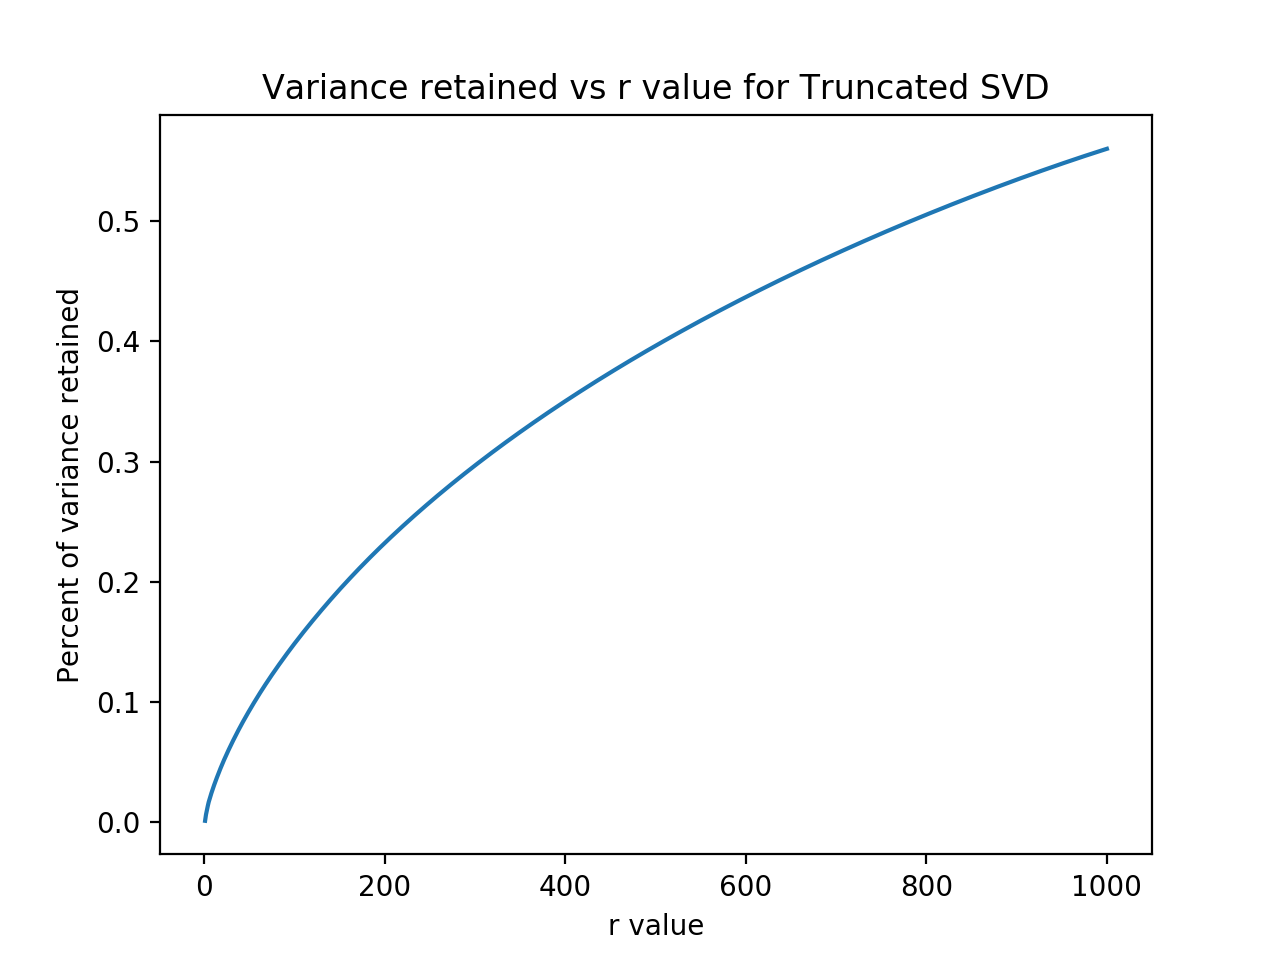
\includegraphics[width=\linewidth]{p3_variance_r.png}
  \vspace*{-20mm}
  \caption{Plot of the Percent of variance retained in PCA vs. r.}
  \label{fig:variance_r}
\end{figure}

For dimensionality reduction, we used LSI and NMF methods. We swept over the parameters for each method (LSI and NMF) to determine the one yielding better results in terms of clustering metrics. All five performance metrics for clustering with different r-values are reported below. \\


\underline{r = 1} \\
\textbf{NMF} \\

Contigency: \[
\begin{bmatrix}
    1744       & 2159\\
    1696       & 2283\\
\end{bmatrix}
\]    
\\ \\

\begin{center}
\begin{tabu}{| c | c | }
\hline
Homogeneity: & 0.000311084586659 \\
\hline
completeness: & 0.00031474279897 \\
\hline
V-measure: & 0.000312903000955 \\
\hline
RAND score: & 0.000349910576703 \\
\hline
Mutual Info: & 0.000219562406476 \\
\hline
\end{tabu}
\end{center}

\textbf{SVD} \\
Contingency: \[
\begin{bmatrix}
 2160			& 1743 \\
 2284 			& 1695 \\
\end{bmatrix}
\]
\\ \\

\begin{center}
\begin{tabu}{| c | c |}
\hline
Homogeneity: & 0.000310977615107 \\
\hline 
completeness: & 0.000314664424341 \\
\hline
V-measure: & 0.000312810156833  \\
\hline
RAND score: & 0.000349914958924  \\
\hline
Mutual Info:  & 0.000219455422027 \\
\hline
\end{tabu}
\end{center}

\underline{r = 2} \\
\textbf{NMF} \\
Contingency: \[
\begin{bmatrix}
 731		& 3172 \\
 3943		& 36 \\
\end{bmatrix}
\]
\\ \\

\begin{center}
\begin{tabu}{ | c | c | }
\hline 
Homogeneity: 	& 0.592844515412 \\
\hline
completeness:	& 0.608067163036 \\
\hline
V-measure: 		& 0.600359358773 \\
\hline
RAND score: 	& 0.648591716894 \\
\hline
Mutual Info:	& 0.592807239875 \\
\hline
\end{tabu}
\end{center}


\textbf{SVD} \\
Contingency: \[
\begin{bmatrix}
250 		& 3653 \\
3618  		& 361 \\
\end{bmatrix}
\]
\\ \\

\begin{center}
\begin{tabu}{| c | c |}
\hline
Homogeneity:		& 0.608223241581 \\
\hline
Completeness:		& 0.608333021975 \\
\hline
V-measure:			& 0.608278126825 \\
\hline
RAND score:			& 0.713926529273 \\
\hline
Mutual Info:		& 0.608187374307 \\
\hline
\end{tabu}
\end{center}


\underline{r = 3} \\
\textbf{NMF} \\
Contingency: \[
\begin{bmatrix}
13 			& 3890 \\
1674		& 2305 \\
\end{bmatrix}
\]

\begin{center}
\begin{tabu}{| c | c |}
\hline
Homogeneity: 		& 0.237561424862 \\
\hline
Completeness: 		& 0.317099662339 \\
\hline
V-measure:			& 0.271627663619 \\
\hline
RAND score: 		& 0.16950318518 \\
\hline
Mutual Info: 		& 0.237491614778 \\
\hline
\end{tabu}
\end{center}

\textbf{SVD} \\

Contingency: \[
\begin{bmatrix}
3635  		& 268 \\
3979    	& 0   \\
\end{bmatrix}
\]
\\ \\

\begin{center}
\begin{tabu}{| c | c |}
\hline
Homogeneity: 		& 0.0353596802034 \\
\hline 
Completeness: 		& 0.165160546781 \\
\hline
V-measure: 			& 0.0582487283625 \\
\hline
RAND score: 		& 0.00593193880668 \\
\hline
Mutual Info: 		& 0.0352712181601 \\
\hline
\end{tabu}
\end{center}

\underlin{r = 5} \\
\textbf{NMF} \\
Contingency: \[ 
\begin{bmatrix}
2992  		& 911 \\
1427	    & 2552 \\
\end{bmatrix}
\]
\\ \\

\begin{center}
\begin{tabu}{| c | c |}
\hline
Homogeneity: 		& 0.125884883543 \\
\hline
Completeness: 		& 0.127229904183 \\
\hline
V-measure: 			& 0.126553820227 \\
\hline
RAND score: 		& 0.165339719484 \\
\hline
Mutual Info: 		& 0.125804857758 \\
\hline
\end{tabu}
\end{center}

\textbf{SVD}\\

Contingency: \[
\begin{bmatrix}
445 		& 3458 \\
2023 		& 1956 \\
\end{bmatrix}
\]
\\ \\

\begin{center}
\begin{tabu}{| c | c |}
\hline
Homogeneity: 		& 0.138545661957 \\
\hline
Completeness: 		& 0.154488808534 \\
\hline
V-measure: 			& 0.146083525309 \\
\hline
RAND score: 		& 0.15259281864 \\
\hline
Mutual Info: 		& 0.13846679232 \\
\hline
\end{tabu}
\end{center}


\underline{r = 10} \\
\textbf{NMF} \\
Contingency: \[
\begin{bmatrix}
1226 		& 2677 \\
3975	    & 4 \\
\end{bmatrix}
\]
\\ \\

\begin{center}
\begin{tabu}{| c | c |}
\hline
Homogeneity: 		& 0.474595160933 \\
\hline
Completeness: 		& 0.513066612395 \\
\hline
V-measure: 			& 0.4930816157 \\
\hline
RAND score: 		& 0.473136537245 \\
\hline
Mutual Info: 		& 0.474547058583 \\
\hline
\end{tabu}
\end{center}


\textbf{SVD} \\
Contingency:\[ 
\begin{bmatrix}
3900    	& 3 \\
2388 		& 1591 \\
\end{bmatrix}
\]
\\ \\

\begin{center}
\begin{tabu}{| c | c |}
\hline
Homogeneity: 		& 0.231788794819 \\
\hline
Completeness: 		& 0.319083600677 \\
\hline
V-measure: 			& 0.268519547729 \\
\hline
RAND score: 		& 0.154588731327 \\
\hline
Mutual Info: 		& 0.23171845505 \\
\hline
\end{tabu}
\end{center}

\underline{r = 20} \\
\textbf{NMF} \\
Contingency: \[
\begin{bmatrix}
3894    	& 9 \\
3154  		& 825 \\
\end{bmatrix}
\]
\\ \\

\begin{center}
\begin{tabu}{| c | c |}
\hline
Homogeneity: 		& 0.103775132137 \\
\hline
Completeness: 		& 0.213011153692 \\
\hline
V-measure: 			& 0.139559454496 \\
\hline
RAND score: 		& 0.0388697375327 \\
\hline
Mutual Info: 		& 0.103693048241 \\
\hline
\end{tabu}
\end{center}

\textbf{SVD} \\
Contingency: \[
\begin{bmatrix}
3 		& 3900 \\
1598 	& 2381 \\
\end{bmatrix}
\]
\\ \\

\begin{center}
\begin{tabu}{| c | c |}
\hline
Homogeneity: 		& 0.233028131747 \\
\hline
Completeness: 		& 0.320016548166 \\
\hline
V-measure: 			& 0.269681134475 \\
\hline
RAND score: 		& 0.155989148922 \\
\hline
Mutual Info: 		& 0.232957905546 \\
\hline
\end{tabu}
\end{center}


\underline{r = 50} \\
\textbf{NMF} \\
Contingency: \[
\begin{bmatrix}
3 		& 3900 \\
530 	& 3449 \\
\end{bmatrix}
\]
\\ \\

\begin{center}
\begin{tabu}{| c | c |}
\hline
Homogeneity: 		& 0.0667025153879 \\
\hline
Completeness: 		& 0.186835673058 \\
\hline
V-measure: 			& 0.0983079466928 \\
\hline
RAND score: 		& 0.0152959218258 \\
\hline
Mutual Info: 		& 0.0666170072715 \\
\hline
\end{tabu}
\end{center}


\textbf{SVD} \\
Contingency: \[
\begin{bmatrix}
211 		& 3692 \\
3896   		& 83 \\
\end{bmatrix}
\]
\\ \\ 


\begin{center}
\begin{tabu}{| c | c |}
\hline
Homogeneity: 		& 0.774707930719  \\
\hline
Completeness: 		& 0.775648956185 \\
\hline
V-measure: 			& 0.775178157863 \\
\hline
RAND score: 		& 0.856346285004 \\
\hline
Mutual Info: 		& 0.774687305158 \\
\hline
\end{tabu}
\end{center}


\underline{ r = 100} \\
\textbf{NMF} \\
Contingency: \[
\begin{bmatrix}
13 		& 3890 \\
13 		& 3966 \\
\end{bmatrix}
\]
\\ \\

\begin{center}
\begin{tabu}{| c | c |}
\hline
Homogeneity: 		& 2.21983210362e-07 \\
\hline
Completeness: 		& 6.94847451879e-06 \\
\hline
V-measure: 			& 4.30222097127e-07 \\
\hline
RAND score: 		& -4.45905813813e-07 \\
\hline
Mutual Info: 		& -9.31724050412e-05  \\
\hline
\end{tabu}
\end{center}


\textbf{SVD} \\
Contingency: \[
\begin{bmatrix}
3900    	& 3 \\
2310	 	& 1669 \\
\end{bmatrix}
\]
\\ \\


\begin{center}
\begin{tabu}{| c | c |}
\hline
Homogeneity: 		& 0.245732969386 \\
\hline
Completeness:  		& 0.329585259245 \\
\hline
V-measure: 			& 0.281548403613 \\
\hline
RAND score: 		& 0.170550013258 \\
\hline
Mutual Info: 		& 0.245663907331 \\
\hline
\end{tabu}
\end{center}


\underline{r = 300} \\
\textbf{NMF} \\
Contingency: \[
\begin{bmatrix} 
3871   		& 32 \\
3889   		& 90 \\ 
\end{bmatrix}
\]
\\ \\


\begin{center}
\begin{tabu}{| c | c |}
\hline
Homogeneity: 		& 0.00256529809666 \\ 
\hline
Completeness: 		& 0.0222595262258 \\
\hline
V-measure: 			& 0.00460042089466 \\
\hline
RAND score: 		& -6.92914675877e-05 \\
\hline
Mutual Info: 		& 0.00247362159362 \\
\hline
\end{tabu}
\end{center}

\textbf{SVD} \\
Contingency: \[
\begin{bmatrix}
55 		& 3848 \\
1846 	& 2133 \\
\end{bmatrix}
\]
\\ \\


\begin{center}
\begin{tabu}{| c | c |}
\hline
Homogeneity: 		& 0.241189275662 \\
\hline
Completeness: 		& 0.302600706133 \\
\hline
V-measure: 			& 0.268427325146 \\
\hline
RAND score: 		& 0.197762294913 \\ 
\hline
Mutual Info: 		& 0.24111979987 \\
\hline
\end{tabu}
\end{center}


\section*{Performance Visualization & Improvement}

\begin{figure}
  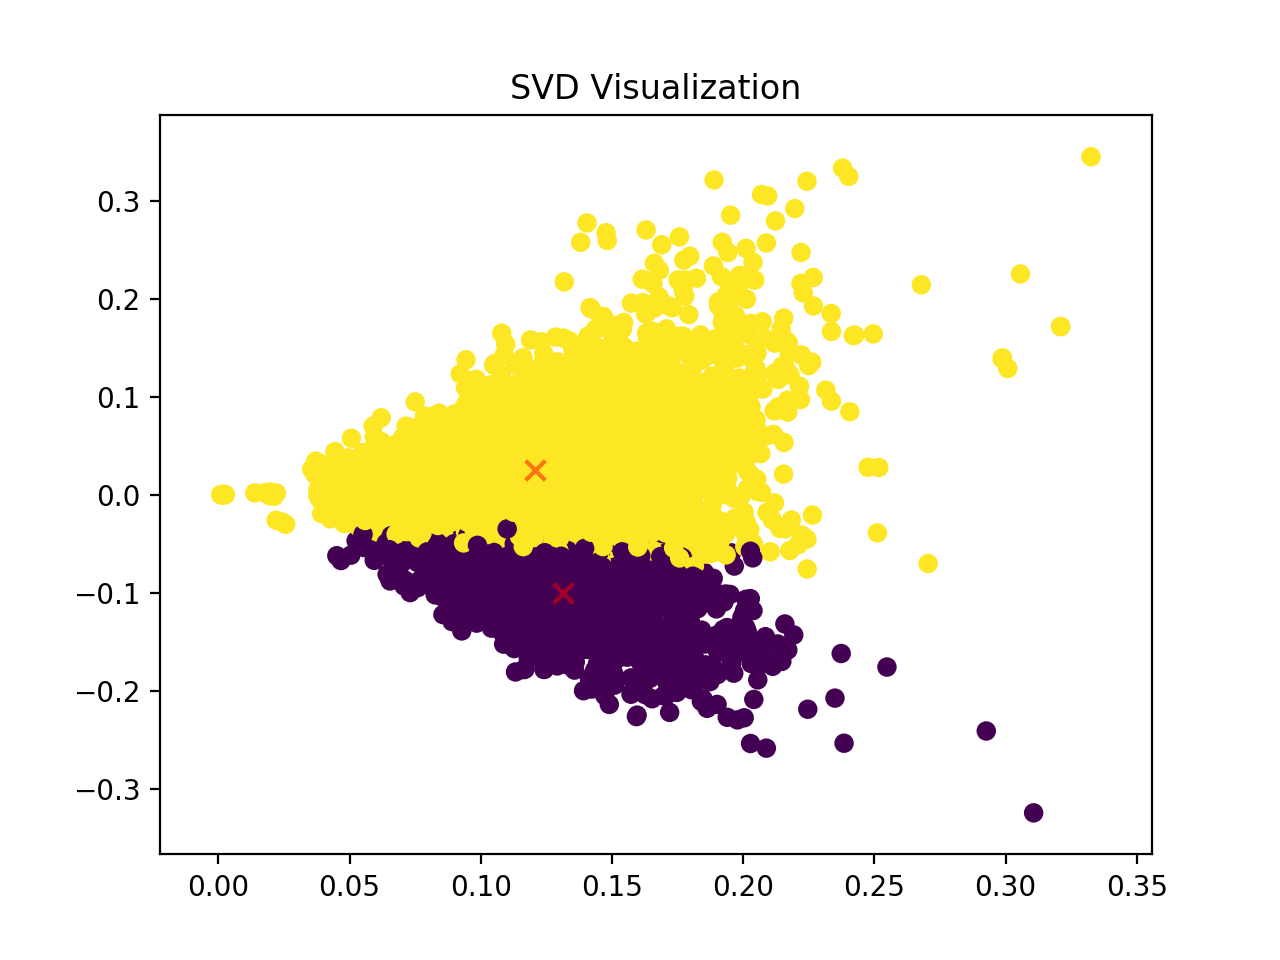
\includegraphics[width=\linewidth]{svd_clusters_4a.png}
	\vspace*{-20mm}  
 
  \caption{Clustering result for SVD with the best r-value}
   \label{fig:svd1}
\end{figure}

\begin{figure}
  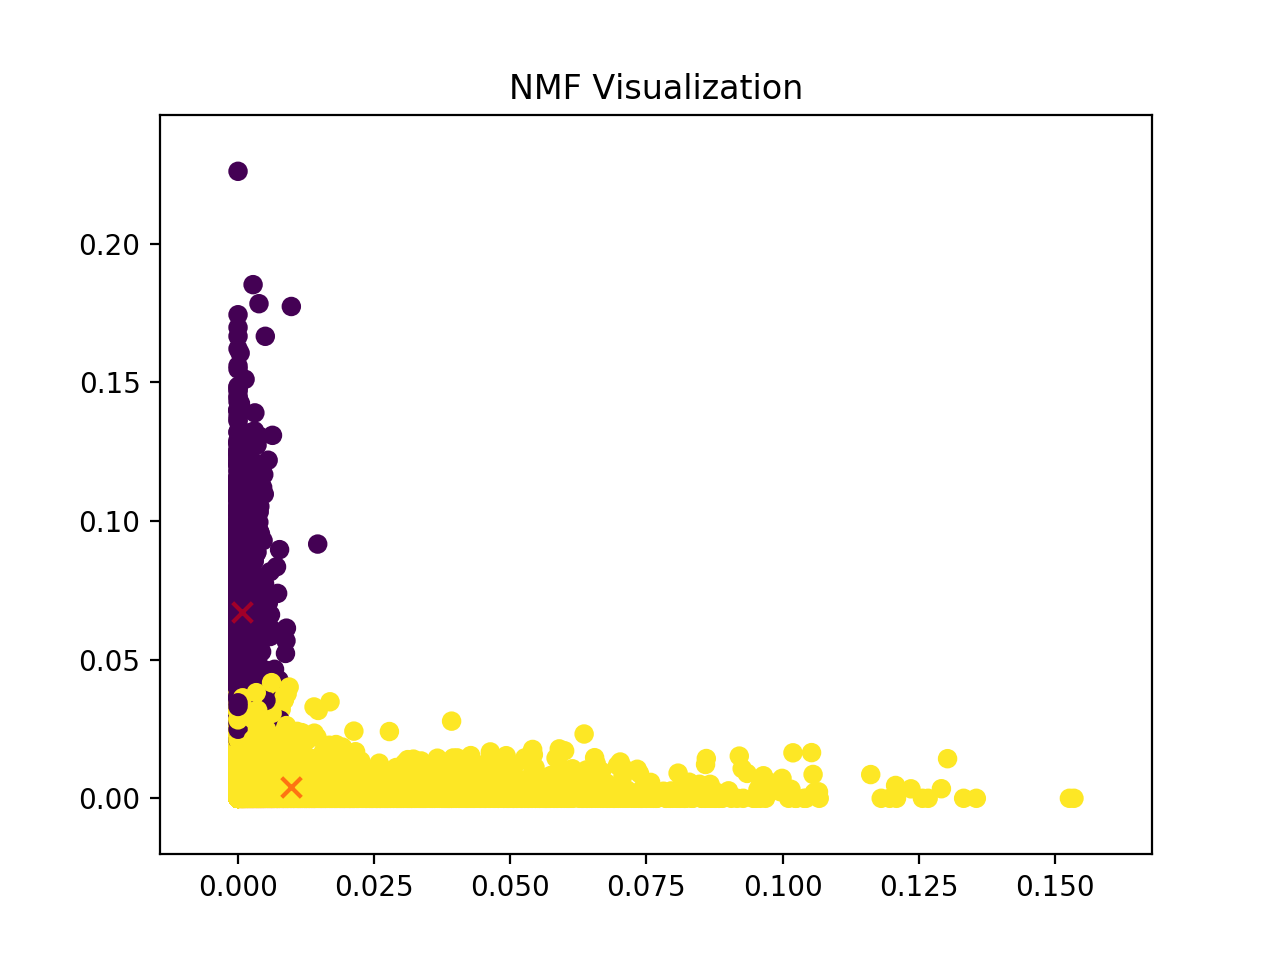
\includegraphics[width=\linewidth]{nmf_clusters_4a.png} 
  \vspace*{-20mm}
  \caption{Clustering result for NMF with the best r-value}
  \label{fig:nmf1}
\end{figure}

By projecting final data vectors onto 2-dimensional plane and color-coding the classes, the best clustering results from previous part for both SVD and NMF have been visualized in \ref[fig:svd1} and \ref{fig:nmf1} figures. 





\end{document}